
%% bare_jrnl.tex
%% V1.4a
%% 2014/09/17
%% by Michael Shell
%% see http://www.michaelshell.org/
%% for current contact information.
%%
%% This is a skeleton file demonstrating the use of IEEEtran.cls
%% (requires IEEEtran.cls version 1.8a or later) with an IEEE
%% journal paper.
%%
%% Support sites:
%% http://www.michaelshell.org/tex/ieeetran/
%% http://www.ctan.org/tex-archive/macros/latex/contrib/IEEEtran/
%% and
%% http://www.ieee.org/

%%*************************************************************************
%% Legal Notice:
%% This code is offered as-is without any warranty either expressed or
%% implied; without even the implied warranty of MERCHANTABILITY or
%% FITNESS FOR A PARTICULAR PURPOSE! 
%% User assumes all risk.
%% In no event shall IEEE or any contributor to this code be liable for
%% any damages or losses, including, but not limited to, incidental,
%% consequential, or any other damages, resulting from the use or misuse
%% of any information contained here.
%%
%% All comments are the opinions of their respective authors and are not
%% necessarily endorsed by the IEEE.
%%
%% This work is distributed under the LaTeX Project Public License (LPPL)
%% ( http://www.latex-project.org/ ) version 1.3, and may be freely used,
%% distributed and modified. A copy of the LPPL, version 1.3, is included
%% in the base LaTeX documentation of all distributions of LaTeX released
%% 2003/12/01 or later.
%% Retain all contribution notices and credits.
%% ** Modified files should be clearly indicated as such, including  **
%% ** renaming them and changing author support contact information. **
%%
%% File list of work: IEEEtran.cls, IEEEtran_HOWTO.pdf, bare_adv.tex,
%%                    bare_conf.tex, bare_jrnl.tex, bare_conf_compsoc.tex,
%%                    bare_jrnl_compsoc.tex, bare_jrnl_transmag.tex
%%*************************************************************************


% *** Authors should verify (and, if needed, correct) their LaTeX system  ***
% *** with the testflow diagnostic prior to trusting their LaTeX platform ***
% *** with production work. IEEE's font choices and paper sizes can       ***
% *** trigger bugs that do not appear when using other class files.       ***                          ***
% The testflow support page is at:
% http://www.michaelshell.org/tex/testflow/



\documentclass[letter]{IEEEtran}
%
% If IEEEtran.cls has not been installed into the LaTeX system files,
% manually specify the path to it like:
% \documentclass[journal]{../sty/IEEEtran}





% Some very useful LaTeX packages include:
% (uncomment the ones you want to load)


% *** MISC UTILITY PACKAGES ***
%
%\usepackage{ifpdf}
% Heiko Oberdiek's ifpdf.sty is very useful if you need conditional
% compilation based on whether the output is pdf or dvi.
% usage:
% \ifpdf
%   % pdf code
% \else
%   % dvi code
% \fi
% The latest version of ifpdf.sty can be obtained from:
% http://www.ctan.org/tex-archive/macros/latex/contrib/oberdiek/
% Also, note that IEEEtran.cls V1.7 and later provides a builtin
% \ifCLASSINFOpdf conditional that works the same way.
% When switching from latex to pdflatex and vice-versa, the compiler may
% have to be run twice to clear warning/error messages.






% *** CITATION PACKAGES ***
%
%\usepackage{cite}
% cite.sty was written by Donald Arseneau
% V1.6 and later of IEEEtran pre-defines the format of the cite.sty package
% \cite{} output to follow that of IEEE. Loading the cite package will
% result in citation numbers being automatically sorted and properly
% "compressed/ranged". e.g., [1], [9], [2], [7], [5], [6] without using
% cite.sty will become [1], [2], [5]--[7], [9] using cite.sty. cite.sty's
% \cite will automatically add leading space, if needed. Use cite.sty's
% noadjust option (cite.sty V3.8 and later) if you want to turn this off
% such as if a citation ever needs to be enclosed in parenthesis.
% cite.sty is already installed on most LaTeX systems. Be sure and use
% version 5.0 (2009-03-20) and later if using hyperref.sty.
% The latest version can be obtained at:
% http://www.ctan.org/tex-archive/macros/latex/contrib/cite/
% The documentation is contained in the cite.sty file itself.






% *** GRAPHICS RELATED PACKAGES ***
%
\ifCLASSINFOpdf
   \usepackage[pdftex]{graphicx}
  % declare the path(s) where your graphic files are
  % \graphicspath{{../pdf/}{../jpeg/}}
  % and their extensions so you won't have to specify these with
  % every instance of \includegraphics
  % \DeclareGraphicsExtensions{.pdf,.jpeg,.png}
\else
  % or other class option (dvipsone, dvipdf, if not using dvips). graphicx
  % will default to the driver specified in the system graphics.cfg if no
  % driver is specified.
  % \usepackage[dvips]{graphicx}
  % declare the path(s) where your graphic files are
  % \graphicspath{{../eps/}}
  % and their extensions so you won't have to specify these with
  % every instance of \includegraphics
  % \DeclareGraphicsExtensions{.eps}
\fi
% graphicx was written by David Carlisle and Sebastian Rahtz. It is
% required if you want graphics, photos, etc. graphicx.sty is already
% installed on most LaTeX systems. The latest version and documentation
% can be obtained at: 
% http://www.ctan.org/tex-archive/macros/latex/required/graphics/
% Another good source of documentation is "Using Imported Graphics in
% LaTeX2e" by Keith Reckdahl which can be found at:
% http://www.ctan.org/tex-archive/info/epslatex/
%
% latex, and pdflatex in dvi mode, support graphics in encapsulated
% postscript (.eps) format. pdflatex in pdf mode supports graphics
% in .pdf, .jpeg, .png and .mps (metapost) formats. Users should ensure
% that all non-photo figures use a vector format (.eps, .pdf, .mps) and
% not a bitmapped formats (.jpeg, .png). IEEE frowns on bitmapped formats
% which can result in "jaggedy"/blurry rendering of lines and letters as
% well as large increases in file sizes.
%
% You can find documentation about the pdfTeX application at:
% http://www.tug.org/applications/pdftex





% *** MATH PACKAGES ***
%
%\usepackage[cmex10]{amsmath}
% A popular package from the American Mathematical Society that provides
% many useful and powerful commands for dealing with mathematics. If using
% it, be sure to load this package with the cmex10 option to ensure that
% only type 1 fonts will utilized at all point sizes. Without this option,
% it is possible that some math symbols, particularly those within
% footnotes, will be rendered in bitmap form which will result in a
% document that can not be IEEE Xplore compliant!
%
% Also, note that the amsmath package sets \interdisplaylinepenalty to 10000
% thus preventing page breaks from occurring within multiline equations. Use:
%\interdisplaylinepenalty=2500
% after loading amsmath to restore such page breaks as IEEEtran.cls normally
% does. amsmath.sty is already installed on most LaTeX systems. The latest
% version and documentation can be obtained at:
% http://www.ctan.org/tex-archive/macros/latex/required/amslatex/math/





% *** SPECIALIZED LIST PACKAGES ***
%
%\usepackage{algorithmic}
% algorithmic.sty was written by Peter Williams and Rogerio Brito.
% This package provides an algorithmic environment fo describing algorithms.
% You can use the algorithmic environment in-text or within a figure
% environment to provide for a floating algorithm. Do NOT use the algorithm
% floating environment provided by algorithm.sty (by the same authors) or
% algorithm2e.sty (by Christophe Fiorio) as IEEE does not use dedicated
% algorithm float types and packages that provide these will not provide
% correct IEEE style captions. The latest version and documentation of
% algorithmic.sty can be obtained at:
% http://www.ctan.org/tex-archive/macros/latex/contrib/algorithms/
% There is also a support site at:
% http://algorithms.berlios.de/index.html
% Also of interest may be the (relatively newer and more customizable)
% algorithmicx.sty package by Szasz Janos:
% http://www.ctan.org/tex-archive/macros/latex/contrib/algorithmicx/




% *** ALIGNMENT PACKAGES ***
%
%\usepackage{array}
% Frank Mittelbach's and David Carlisle's array.sty patches and improves
% the standard LaTeX2e array and tabular environments to provide better
% appearance and additional user controls. As the default LaTeX2e table
% generation code is lacking to the point of almost being broken with
% respect to the quality of the end results, all users are strongly
% advised to use an enhanced (at the very least that provided by array.sty)
% set of table tools. array.sty is already installed on most systems. The
% latest version and documentation can be obtained at:
% http://www.ctan.org/tex-archive/macros/latex/required/tools/


% IEEEtran contains the IEEEeqnarray family of commands that can be used to
% generate multiline equations as well as matrices, tables, etc., of high
% quality.




% *** SUBFIGURE PACKAGES ***
%\ifCLASSOPTIONcompsoc
%  \usepackage[caption=false,font=normalsize,labelfont=sf,textfont=sf]{subfig}
%\else
%  \usepackage[caption=false,font=footnotesize]{subfig}
%\fi
% subfig.sty, written by Steven Douglas Cochran, is the modern replacement
% for subfigure.sty, the latter of which is no longer maintained and is
% incompatible with some LaTeX packages including fixltx2e. However,
% subfig.sty requires and automatically loads Axel Sommerfeldt's caption.sty
% which will override IEEEtran.cls' handling of captions and this will result
% in non-IEEE style figure/table captions. To prevent this problem, be sure
% and invoke subfig.sty's "caption=false" package option (available since
% subfig.sty version 1.3, 2005/06/28) as this is will preserve IEEEtran.cls
% handling of captions.
% Note that the Computer Society format requires a larger sans serif font
% than the serif footnote size font used in traditional IEEE formatting
% and thus the need to invoke different subfig.sty package options depending
% on whether compsoc mode has been enabled.
%
% The latest version and documentation of subfig.sty can be obtained at:
% http://www.ctan.org/tex-archive/macros/latex/contrib/subfig/




% *** FLOAT PACKAGES ***
%
%\usepackage{fixltx2e}
% fixltx2e, the successor to the earlier fix2col.sty, was written by
% Frank Mittelbach and David Carlisle. This package corrects a few problems
% in the LaTeX2e kernel, the most notable of which is that in current
% LaTeX2e releases, the ordering of single and double column floats is not
% guaranteed to be preserved. Thus, an unpatched LaTeX2e can allow a
% single column figure to be placed prior to an earlier double column
% figure. The latest version and documentation can be found at:
% http://www.ctan.org/tex-archive/macros/latex/base/


%\usepackage{stfloats}
% stfloats.sty was written by Sigitas Tolusis. This package gives LaTeX2e
% the ability to do double column floats at the bottom of the page as well
% as the top. (e.g., "\begin{figure*}[!b]" is not normally possible in
% LaTeX2e). It also provides a command:
%\fnbelowfloat
% to enable the placement of footnotes below bottom floats (the standard
% LaTeX2e kernel puts them above bottom floats). This is an invasive package
% which rewrites many portions of the LaTeX2e float routines. It may not work
% with other packages that modify the LaTeX2e float routines. The latest
% version and documentation can be obtained at:
% http://www.ctan.org/tex-archive/macros/latex/contrib/sttools/
% Do not use the stfloats baselinefloat ability as IEEE does not allow
% \baselineskip to stretch. Authors submitting work to the IEEE should note
% that IEEE rarely uses double column equations and that authors should try
% to avoid such use. Do not be tempted to use the cuted.sty or midfloat.sty
% packages (also by Sigitas Tolusis) as IEEE does not format its papers in
% such ways.
% Do not attempt to use stfloats with fixltx2e as they are incompatible.
% Instead, use Morten Hogholm'a dblfloatfix which combines the features
% of both fixltx2e and stfloats:
%
% \usepackage{dblfloatfix}
% The latest version can be found at:
% http://www.ctan.org/tex-archive/macros/latex/contrib/dblfloatfix/




%\ifCLASSOPTIONcaptionsoff
%  \usepackage[nomarkers]{endfloat}
% \let\MYoriglatexcaption\caption
% \renewcommand{\caption}[2][\relax]{\MYoriglatexcaption[#2]{#2}}
%\fi
% endfloat.sty was written by James Darrell McCauley, Jeff Goldberg and 
% Axel Sommerfeldt. This package may be useful when used in conjunction with 
% IEEEtran.cls'  captionsoff option. Some IEEE journals/societies require that
% submissions have lists of figures/tables at the end of the paper and that
% figures/tables without any captions are placed on a page by themselves at
% the end of the document. If needed, the draftcls IEEEtran class option or
% \CLASSINPUTbaselinestretch interface can be used to increase the line
% spacing as well. Be sure and use the nomarkers option of endfloat to
% prevent endfloat from "marking" where the figures would have been placed
% in the text. The two hack lines of code above are a slight modification of
% that suggested by in the endfloat docs (section 8.4.1) to ensure that
% the full captions always appear in the list of figures/tables - even if
% the user used the short optional argument of \caption[]{}.
% IEEE papers do not typically make use of \caption[]'s optional argument,
% so this should not be an issue. A similar trick can be used to disable
% captions of packages such as subfig.sty that lack options to turn off
% the subcaptions:
% For subfig.sty:
% \let\MYorigsubfloat\subfloat
% \renewcommand{\subfloat}[2][\relax]{\MYorigsubfloat[]{#2}}
% However, the above trick will not work if both optional arguments of
% the \subfloat command are used. Furthermore, there needs to be a
% description of each subfigure *somewhere* and endfloat does not add
% subfigure captions to its list of figures. Thus, the best approach is to
% avoid the use of subfigure captions (many IEEE journals avoid them anyway)
% and instead reference/explain all the subfigures within the main caption.
% The latest version of endfloat.sty and its documentation can obtained at:
% http://www.ctan.org/tex-archive/macros/latex/contrib/endfloat/
%
% The IEEEtran \ifCLASSOPTIONcaptionsoff conditional can also be used
% later in the document, say, to conditionally put the References on a 
% page by themselves.




% *** PDF, URL AND HYPERLINK PACKAGES ***
%
\usepackage{url}
% url.sty was written by Donald Arseneau. It provides better support for
% handling and breaking URLs. url.sty is already installed on most LaTeX
% systems. The latest version and documentation can be obtained at:
% http://www.ctan.org/tex-archive/macros/latex/contrib/url/
% Basically, \url{my_url_here}.




% *** Do not adjust lengths that control margins, column widths, etc. ***
% *** Do not use packages that alter fonts (such as pslatex).         ***
% There should be no need to do such things with IEEEtran.cls V1.6 and later.
% (Unless specifically asked to do so by the journal or conference you plan
% to submit to, of course. )


% correct bad hyphenation here
\usepackage{amsmath}
\hyphenation{op-tical net-works semi-conduc-tor}
\usepackage{pdflscape}
\usepackage{arydshln}
\usepackage{epstopdf}
\usepackage{booktabs}


\begin{document}
%
% paper title
% Titles are generally capitalized except for words such as a, an, and, as,
% at, but, by, for, in, nor, of, on, or, the, to and up, which are usually
% not capitalized unless they are the first or last word of the title.
% Linebreaks \\ can be used within to get better formatting as desired.
% Do not put math or special symbols in the title.
\title{A Guide to Solar Power Forecasting using ARMA Models}
\title{Solar Power Forecasting using ARMA Models}
%
%
% author names and IEEE memberships
% note positions of commas and nonbreaking spaces ( ~ ) LaTeX will not break
% a structure at a ~ so this keeps an author's name from being broken across
% two lines.
% use \thanks{} to gain access to the first footnote area
% a separate \thanks must be used for each paragraph as LaTeX2e's \thanks
% was not built to handle multiple paragraphs
%

\author{Bismark~Singh, and~David~Pozo,~\IEEEmembership{Member,~IEEE}
\thanks{B.~Singh is with the Discrete Mathematics \& Optimization, Sandia 
National Laboratories, Albuquerque, NM 87185, USA
e-mail: bsingh@sandia.gov.}% <-this % stops a space
\thanks{D.~Pozo is with the Center for Energy Systems, Skolkovo Institute of 
Science and Technology, Moscow, Russia.}}% <-this 
% stops a space
%\thanks{Manuscript received April 19, 2005; revised September 17, 2014.}}

% note the % following the last \IEEEmembership and also \thanks - 
% these prevent an unwanted space from occurring between the last author name
% and the end of the author line. i.e., if you had this:
% 
% \author{....lastname \thanks{...} \thanks{...} }
%                     ^------------^------------^----Do not want these spaces!
%
% a space would be appended to the last name and could cause every name on that
% line to be shifted left slightly. This is one of those "LaTeX things". For
% instance, "\textbf{A} \textbf{B}" will typeset as "A B" not "AB". To get
% "AB" then you have to do: "\textbf{A}\textbf{B}"
% \thanks is no different in this regard, so shield the last } of each \thanks
% that ends a line with a % and do not let a space in before the next \thanks.
% Spaces after \IEEEmembership other than the last one are OK (and needed) as
% you are supposed to have spaces between the names. For what it is worth,
% this is a minor point as most people would not even notice if the said evil
% space somehow managed to creep in.



% The paper headers
\markboth{Journal of \LaTeX\ Class Files,~Vol.~13, No.~9, September~2014}%
{Shell \MakeLowercase{\textit{et al.}}: Bare Demo of IEEEtran.cls for Journals}
% The only time the second header will appear is for the odd numbered pages
% after the title page when using the twoside option.
% 
% *** Note that you probably will NOT want to include the author's ***
% *** name in the headers of peer review papers.                   ***
% You can use \ifCLASSOPTIONpeerreview for conditional compilation here if
% you desire.




% If you want to put a publisher's ID mark on the page you can do it like
% this:
%\IEEEpubid{0000--0000/00\$00.00~\copyright~2014 IEEE}
% Remember, if you use this you must call \IEEEpubidadjcol in the second
% column for its text to clear the IEEEpubid mark.



% use for special paper notices
%\IEEEspecialpapernotice{(Invited Paper)}




% make the title area
\maketitle

% As a general rule, do not put math, special symbols or citations
% in the abstract or keywords.
\begin{abstract}
	In this letter, we describe a simple and succinct methodology to develop hourly auto-regressive 
	moving average (ARMA) model to forecast power output from a photovoltaic solar generator. 
	We illustrate how to build the  model, to use  statistical tests, to validate it, and construct hourly samples. 
	While the resulting model inherits nice properties for embedding into more sophisticated operation and planning models, it shows at the same time, relative good accuracy. Additionally, it represents a good forecasting tool for sample generation for stochastic energy optimization models.
\end{abstract}

% Note that keywords are not normally used for peerreview papers.
\begin{IEEEkeywords}
ARMA, solar power, photovoltaic, forecasting, scenario generation
\end{IEEEkeywords}






% For peer review papers, you can put extra information on the cover
% page as needed:
% \ifCLASSOPTIONpeerreview
% \begin{center} \bfseries EDICS Category: 3-BBND \end{center}
% \fi
%
% For peerreview papers, this IEEEtran command inserts a page break and
% creates the second title. It will be ignored for other modes.
\IEEEpeerreviewmaketitle



\section{Introduction}
\IEEEPARstart{I}{ncreasing} penetration of renewable energy sources, such as wind and solar, in 
the electricity grid requires an accurate representation of the 
uncertainty to guarantee feasibility of the system operations, and 
for efficiently planning new transmission lines and generation capacities. To 
address these challenges, advanced decision-making models that lie at the
interface of statistics and operation research fields have been widely 
explored.  Representation of the  uncertainty in renewable energy is typically  
done by either using \textit{samples} or a  \textit{set representation} from the 
underlying stochastic process. The former generally requires forecasting tools 
for generating synthetic samples or scenarios that are used for feeding 
decision-making optimization models~\cite{kleywegt2002sample}. The latter 
requires a simple representation of the stochastic process in 
order to embed it into more sophisticated decision-making 
tools~\cite{lorca2015adaptive}. In both cases, but especially so in the latter, 
complex forecasting models result in models that are hard to integrate. 

In this letter, we present a forecasting model that is easy-to-embed into more 
sophisticated decision-making models, which at the same time also serves as a 
tool for generating samples of renewable energy forecasts.  In 
particular, we focus on 
forecasting  hourly photovoltaic  (PV) solar power generation, but the 
methodology is not 
limited to this technology.  Solar power differs from wind power due 
to its diurnal nature, and can have much greater  ramps than 
wind~\cite{graabak2016variability}. 

Forecasting methods for solar power are broadly divided 
into two categories: (i) physics-based models---these models predict solar 
power 
from numerical weather predictions and solar irradiation data, and (ii) 
statistical models---these 
models forecast 
solar power directly from historical data. Comparisons of these two 
methods are available; see, 
e.g.,~\cite{huang2010comparative,inman2013solar}. There are other 
approaches available as well which combine these two 
methods~\cite{dong2015novel}. 
In this paper, we center on  statistical  methods alone, and specifically the 
use of auto-regressive moving average (ARMA) 
models to develop our forecasts. 

Despite 
their limitations~\cite{yang2018history}, ARMA models
are widely used to forecast wind power~\cite{brown1984time, 
	duran2007short}, as well as solar 
power~\cite{mora1998multiplicative,yang2012hourly}, because of their ease of 
implementation and parameter selection.  Yet, accurate and 
fast methods to generate solar power scenarios are often unavailable or 
significantly complex, and normal approximations are frequently used; see, 
e.g.,~\cite{su2014stochastic}. 
Here, 
we describe a summary of the methodology to forecast solar power using 
ARMA models. The software codes and generated scenarios are 
available on request. The presented models can 
be applied either to a local PV generating plant or  at the regional 
level.

The main contribution of this letter is to provide a step-by-step approach and 
easy-to-implement ARMA model to forecast PV solar power generation. The 
proposed model is able to capture the important statistical features of the 
parameters, while maintaining simplicity. The model allows modelers to embed
it into more complex decision-making structures, statisticians to have an 
all-in-one place ARMA model design for PV power generation, and policymakers and electrical engineers to have a scenario generation tool. 

\section{Methodology} \label{sec:methodology}

We take hourly year-long historical solar power output 
from a site described in~\cite{golestaneh2016generation}. 
This zone has an altitude of 595m, a nominal power of 1560~MW, a panel 
tilt 
of $36^\circ$, and a $38^\circ$ clockwise panel orientation from the north. 
Further installation specifics are available in zone~1 from Table~1 
of~\cite{golestaneh2016generation}, while technical specifications are 
available 
in~\cite{technical}.  We use approximately nine months of data 
for training. The data does not have any solar power for the ten hours 
[20:00-5:00], and hence we restrict the forecasts in these hours to be zero as 
well. Equivalently, a criteria based on the solar zenith angle can be used; 
i.e., $0^\circ$ at sunrise and $90^\circ$ when the sun is directly overhead. 
For 
each of the remaining 14 hours of the day, we build an ARMA$(p,q)$ 
model. One limitation of this approach is that it does not capture the 
correlations between different hours; see, e.g.,~\cite{pedro2012assessment}. 
For each hour, we verify the stationarity of the time 
series and test a number of ARMA($p,q$) models to find the best 
one. We use statistical tests on the residuals to validate the models. Finally, 
we use Monte Carlo sampling from the best ARMA model, for each hour, to create 
hourly scenarios. Below we provide more details.

\subsection{The ARMA model} \label{sec:arma}

We recall here to the general formulation of  ARMA models for modeling time 
series.  Given a time series $x_t$, we can model the level of its current 
observation depending on the level of its $p$ lagged observations, 
$x_{t-1},x_{t-2}, \ldots, x_{t-p}$, plus an additional white noise error term 
$\epsilon_t$. This model is known as an \textit{autoregressive} model of order 
${p}$, AR($p$):

\begin{equation}\label{eq1}
x_t = \sum_{i=1}^p  \phi_i x_{t-i}   + \epsilon_t
\end{equation}

Next, assume that the level of the current observation is affected not only 
by the current white noise error term, but also by the previous 
$q$ white noise errors. This model is known as a \textit{moving average} 
model of order $q$, MA($q$): 

\begin{equation} \label{eq2}
x_t = \epsilon_t + \sum_{i=1}^q  \theta_i \epsilon_{t-i}   
\end{equation}

An ARMA($p,q$) model combines both equations~\eqref{eq1} and~\eqref{eq2}. 
Observe that the output variable depends linearly on the current and various 
past values (which is an advantage compared to other high fidelity 
forecasting models). An important question is how many 
representative lagged observations should be considered in order to have good 
fidelity while keeping the model as simple as possible. We discuss this in the 
proceeding sections.

\begin{equation}\label{eq3}
x_t =  \sum_{i=1}^p  \phi_i x_{t-i}    + \epsilon_t + \sum_{i=1}^q  \theta_i \epsilon_{t-i}   
\end{equation}

\subsection{Stationarity} \label{sec:stationarity}
An ARMA model may be a suitable forecasting tool if a time-series is 
stationary. We test 
the hourly data for stationarity using the Augmented 
Dickey-Fuller (ADF) test~\cite{dickey1979distribution}. The ADF test has a null 
hypothesis that the series includes a unit root (or, is non-stationary). We 
reject the null hypothesis at a level 0.05 if the test-statistic exceeds its 
0.95 level quantile. For all the 14 hours of the day, the null hypothesis is 
rejected suggesting the series may be stationary, and hence an ARMA model may 
be suitable. If the series were not stationary, an ARIMA model may be suitable; 
see, e.g., \cite{contreras2003arima}.

\subsection{Selecting parameters of the ARMA model} 
Next, we estimate the parameters of the ARMA model, $p$, the order of the 
autoregressive part and, $q$, the order of the moving average part. For each 
hour, we construct 16 models with both $p$ and $q$ between one and four, and 
compute 
the log-likelihood objective function value. Next, for each hour, we calculate 
the Bayesian information criteria (BIC) for the 16 models using $p + q + 1$ 
parameters.  The BIC penalizes for models with more parameters, and the 
smallest value of the BIC gives the best model, for each 
hour. Table~\ref{tab:order} provides our estimated $p$ and $q$  values for 
the 14 hours of the day. We note that none of the hours have an order value 
exceeding two.

\begin{table}[!htb]
	\centering
	\caption{Estimated $p$ and $q$ values for ARMA($p,q$) models for 14 hours of 
		the day}
	\label{tab:order}
	\scalebox{0.8}{
		\begin{tabular}{c| cccccccccccccc}
			\hline 
			Hour & 6:00 & 7:00 & 8:00 & 9:00 & 10:00 & 11:00 & 12:00 \\ \hline
			p       & 1      & 1       & 1      & 1      & 2        & 1       & 1     \\
			q       & 1     & 1        & 1      & 1      & 1         & 1       & 2     \\ \hline
			
			& 13:00 & 14:00 & 15:00 & 16:00 & 17:00 & 18:00 & 19:00 \\ \hline
		    p      & 1     & 1     & 1  & 1     & 1     & 2     & 1   \\
			q	  & 1     & 1   & 1         & 1      & 1     & 1          & 2     \\ \hline
			
			
	\end{tabular}}
\end{table}

\subsection{Prediction}

Figure~\ref{fig:prediction} plots a day-ahead prediction using the above 
constructed ARMA models; i.e., one hour ahead predictions from the 14 ARMA 
models. A number of metrics are available to evaluate the prediction; see, 
e.g.,~\cite{coimbra2013overview}. We use a few of them here. The mean absolute 
error between the actual 
and the predicted series is 
39.6 MW, or  3.3\% of the maximum actual value. The root mean square 
error between the actual and the predicted series is 
61.0 MW, or  5.1\% of the maximum actual value. 

We further verify autocorrelation in the series, for each hour, using the 
Ljung-Box test~\cite{ljung1978measure} on the residuals for lags of 5, 10, 
and 15. The Ljung-Box  test has a 
null hypothesis that the residuals are uncorrelated up to a 
given lag. We reject the null hypothesis at a level 0.05 if its test-statistic 
exceeds its 0.95 level quantile. For all the 14 hours of the day, the null hypothesis is not
rejected suggesting a zero autocorrelation in the series, or the 
model choice may be appropriate. 


\begin{figure}[!t]
	\centering
	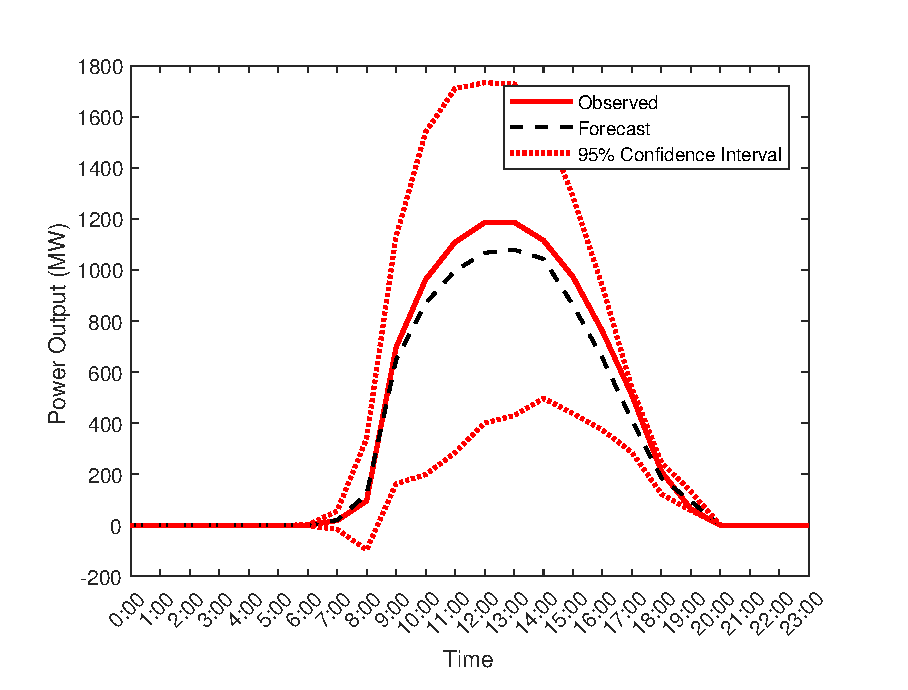
\includegraphics[width=0.5\textwidth]{prediction.eps}
	\caption{Day-ahead actual and predicted values using ARMA models from 
		Table~\ref{tab:order}}
	\label{fig:prediction}
\end{figure}

With increasing penetration of solar power in the electricity grid, a number of 
stochastic optimization models for bidding, storage, and generation have been 
developed; see, e.g.,~\cite{banos2011optimization,sharma2012stochastic}. 
Stochastic optimization models rely on the availability of a large number of 
scenarios.  We can use Monte Carlo sampling to generate hourly solar power 
scenarios. The output from an ARMA model is real valued, and hence can be 
negative. In our analysis, we truncate the negative powered outputs to 0. For 
the 14 hours of 
the day, this sampling resulted in 1.6\% of the outputs with estimated power 
output below -5MW. Figure~\ref{fig:sample} plots 2000 day-ahead scenarios 
as well as the median and 10 percentile values. 


\begin{figure}[!t]
	\centering
	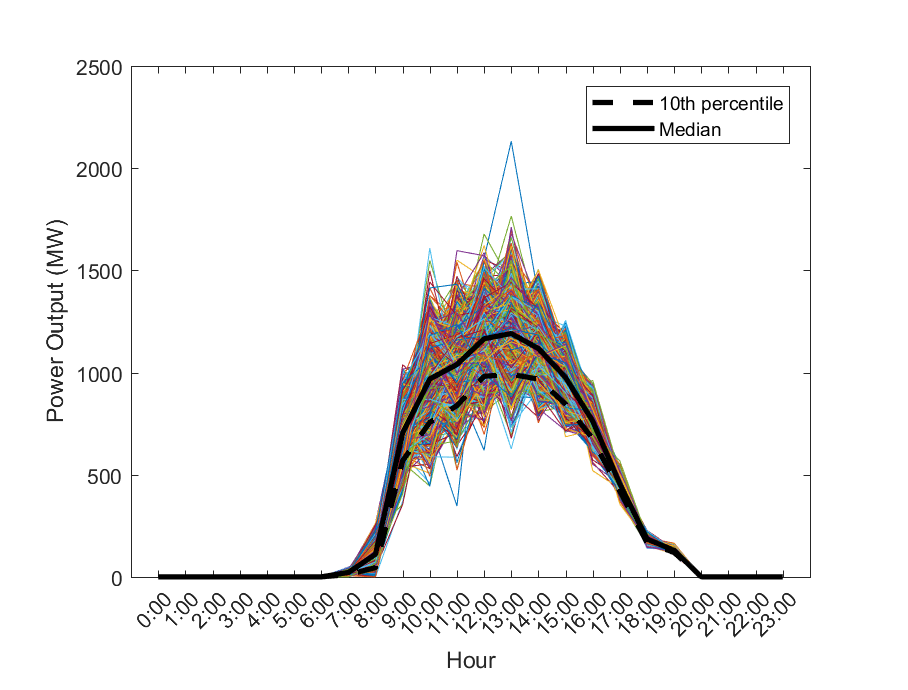
\includegraphics[width=0.5\textwidth]{sample_smooth.eps}
	\caption{2000 hourly scenarios for solar power generated using the ARMA models 
		from Table~\ref{tab:order}. The dashed black line is the median hourly value, 
		and the solid black line is
		the 10 percentile solar power value.}
	\label{fig:sample}
\end{figure}

\section{Conclusions}
In this letter, we present a simple step-by-step scheme for fitting an ARMA 
model to 
historical solar power data. The proposed model provides an easy-to-implement 
linear tool to forecast future hourly scenarios, or for embedding into 
decision-making models. 
We introduce statistical tests to check the applicability of various models, 
identify model parameters, and to finally forecast scenarios. If significant  statistical evidence is not present in support of a  test, the chosen model is not expected to perform well. This can lead to 
erroneous conclusions; see, 
e.g.,~\cite{kwiatkowski1992testing,phillips1988testing}. 
The proposed ARMA model performs better than a Smart-Persistence model (see Appendix). 
In summary, the methodology in this letter can be directly applied to historical data,  both for a single PV source and a PV site,
%to analyze if an ARMA model might be suitable, and can be used  
to create future scenarios for use in stochastic or robust optimization models 
for power system operation and planning. 


\section*{Appendix} \label{sec:appendix}

We compare the developed model against two other forecasting methods. First, we 
fit a single ARMA model, as opposed to hour-by-hour, on the entire time series. 
Second, we use the Smart-Persistence model of~\cite{lauret2016solar}, which 
assumes the solar power at hour $t$ is the mean of the previous $h$ hours. We 
use $h=2$ in here.
Table~\ref{tab:compare} compares the three models; the proposed model performs 
better in both of the chosen metrics. 

\begin{table}[h!]
	\centering
	\caption{Comparison of three forecasting models. MAE denotes the mean absolute 
		error and RMSE denotes the root mean squared error.}
	\label{tab:compare}
	\begin{tabular}{c|ccc}
		\toprule
		\multicolumn{1}{l}{} & \multicolumn{3}{c}{Model}              \\ \hline
		& Hourly ARMA & Single ARMA & Smart-Pers \\ \hline
		MAE (MW)                 & 39.6        & 48.2        & 45.7   \\
		RMSE (MW)                & 61          & 112.51      & 102.6   \\ \bottomrule
	\end{tabular}
\end{table}


%\section*{Acknowledgments} 
%B.\ Singh thanks Jean-Paul Watson and Andrea Staid for helpful discussions and for sharing data. B.\ Singh's work was supported in part by Sandia's Laboratory Directed Research and Development (LDRD) program.
%Sandia National Laboratories is a multimission laboratory managed and operated 
%by National Technology and Engineering Solutions of Sandia, LLC., a wholly owned
%subsidiary of Honeywell International, Inc., for the U.S. Department of 
%Energy's 
%National Nuclear Security Administration under contract DE-NA-0003525. This paper describes objective technical results and analysis. Any subjective 
%views or opinions that might be expressed in the paper do not necessarily 
%represent the views of the U.S. Department of Energy or the United States 
%Government. 
%D.\ Pozo's work was supported by Skoltech NGP Program (Skoltech-MIT joint 
%project).
%


% Can use something like this to put references on a page
% by themselves when using endfloat and the captionsoff option.
\ifCLASSOPTIONcaptionsoff
  \newpage
\fi


% trigger a \newpage just before the given reference
% number - used to balance the columns on the last page
% adjust value as needed - may need to be readjusted if
% the document is modified later
%\IEEEtriggeratref{8}
% The "triggered" command can be changed if desired:
%\IEEEtriggercmd{\enlargethispage{-5in}}

% references section

% can use a bibliography generated by BibTeX as a .bbl file
% BibTeX documentation can be easily obtained at:
% http://www.ctan.org/tex-archive/biblio/bibtex/contrib/doc/
% The IEEEtran BibTeX style support page is at:
% http://www.michaelshell.org/tex/ieeetran/bibtex/
\bibliographystyle{IEEEtran}
\bibliography{mybibfile}
% argument is your BibTeX string definitions and bibliography database(s)
%\bibliography{IEEEabrv,../bib/paper}
%
% <OR> manually copy in the resultant .bbl file
% set second argument of \begin to the number of references
% (used to reserve space for the reference number labels box)


% biography section
% 
% If you have an EPS/PDF photo (graphicx package needed) extra braces are
% needed around the contents of the optional argument to biography to prevent
% the LaTeX parser from getting confused when it sees the complicated
% \includegraphics command within an optional argument. (You could create
% your own custom macro containing the \includegraphics command to make things
% simpler here.)
%\begin{IEEEbiography}[{\includegraphics[width=1in,height=1.25in,clip,keepaspectratio]{mshell}}]{Michael Shell}
% or if you just want to reserve a space for a photo:

%\begin{IEEEbiographynophoto}{Bismark Singh}
%received the B.Tech.\ degree in chemical engineering from the Indian Institute 
%of Technology (IIT), Delhi, India in 2011, the M.S.E.\ and Ph.D.\ degrees in 
%operations 
%research and industrial engineering from The University of Texas at 
%Austin, Austin, TX, USA in 2013 and 2016, respectively. He is currently a 
%postdoctoral appointee at Sandia National Laboratories in Albuquerque, New 
%Mexico, USA.
%\end{IEEEbiographynophoto}
%
%% if you will not have a photo at all:
%\begin{IEEEbiographynophoto}{David Pozo}
%\end{IEEEbiographynophoto}


% You can push biographies down or up by placing
% a \vfill before or after them. The appropriate
% use of \vfill depends on what kind of text is
% on the last page and whether or not the columns
% are being equalized.

%\vfill

% Can be used to pull up biographies so that the bottom of the last one
% is flush with the other column.
%\enlargethispage{-5in}



% that's all folks
\end{document}


